% Options for packages loaded elsewhere
\PassOptionsToPackage{unicode}{hyperref}
\PassOptionsToPackage{hyphens}{url}
%
\documentclass[
]{article}
\usepackage{amsmath,amssymb}
\usepackage{iftex}
\ifPDFTeX
  \usepackage[T1]{fontenc}
  \usepackage[utf8]{inputenc}
  \usepackage{textcomp} % provide euro and other symbols
\else % if luatex or xetex
  \usepackage{unicode-math} % this also loads fontspec
  \defaultfontfeatures{Scale=MatchLowercase}
  \defaultfontfeatures[\rmfamily]{Ligatures=TeX,Scale=1}
\fi
\usepackage{lmodern}
\ifPDFTeX\else
  % xetex/luatex font selection
\fi
% Use upquote if available, for straight quotes in verbatim environments
\IfFileExists{upquote.sty}{\usepackage{upquote}}{}
\IfFileExists{microtype.sty}{% use microtype if available
  \usepackage[]{microtype}
  \UseMicrotypeSet[protrusion]{basicmath} % disable protrusion for tt fonts
}{}
\makeatletter
\@ifundefined{KOMAClassName}{% if non-KOMA class
  \IfFileExists{parskip.sty}{%
    \usepackage{parskip}
  }{% else
    \setlength{\parindent}{0pt}
    \setlength{\parskip}{6pt plus 2pt minus 1pt}}
}{% if KOMA class
  \KOMAoptions{parskip=half}}
\makeatother
\usepackage{xcolor}
\usepackage[margin=1in]{geometry}
\usepackage{color}
\usepackage{fancyvrb}
\newcommand{\VerbBar}{|}
\newcommand{\VERB}{\Verb[commandchars=\\\{\}]}
\DefineVerbatimEnvironment{Highlighting}{Verbatim}{commandchars=\\\{\}}
% Add ',fontsize=\small' for more characters per line
\usepackage{framed}
\definecolor{shadecolor}{RGB}{248,248,248}
\newenvironment{Shaded}{\begin{snugshade}}{\end{snugshade}}
\newcommand{\AlertTok}[1]{\textcolor[rgb]{0.94,0.16,0.16}{#1}}
\newcommand{\AnnotationTok}[1]{\textcolor[rgb]{0.56,0.35,0.01}{\textbf{\textit{#1}}}}
\newcommand{\AttributeTok}[1]{\textcolor[rgb]{0.13,0.29,0.53}{#1}}
\newcommand{\BaseNTok}[1]{\textcolor[rgb]{0.00,0.00,0.81}{#1}}
\newcommand{\BuiltInTok}[1]{#1}
\newcommand{\CharTok}[1]{\textcolor[rgb]{0.31,0.60,0.02}{#1}}
\newcommand{\CommentTok}[1]{\textcolor[rgb]{0.56,0.35,0.01}{\textit{#1}}}
\newcommand{\CommentVarTok}[1]{\textcolor[rgb]{0.56,0.35,0.01}{\textbf{\textit{#1}}}}
\newcommand{\ConstantTok}[1]{\textcolor[rgb]{0.56,0.35,0.01}{#1}}
\newcommand{\ControlFlowTok}[1]{\textcolor[rgb]{0.13,0.29,0.53}{\textbf{#1}}}
\newcommand{\DataTypeTok}[1]{\textcolor[rgb]{0.13,0.29,0.53}{#1}}
\newcommand{\DecValTok}[1]{\textcolor[rgb]{0.00,0.00,0.81}{#1}}
\newcommand{\DocumentationTok}[1]{\textcolor[rgb]{0.56,0.35,0.01}{\textbf{\textit{#1}}}}
\newcommand{\ErrorTok}[1]{\textcolor[rgb]{0.64,0.00,0.00}{\textbf{#1}}}
\newcommand{\ExtensionTok}[1]{#1}
\newcommand{\FloatTok}[1]{\textcolor[rgb]{0.00,0.00,0.81}{#1}}
\newcommand{\FunctionTok}[1]{\textcolor[rgb]{0.13,0.29,0.53}{\textbf{#1}}}
\newcommand{\ImportTok}[1]{#1}
\newcommand{\InformationTok}[1]{\textcolor[rgb]{0.56,0.35,0.01}{\textbf{\textit{#1}}}}
\newcommand{\KeywordTok}[1]{\textcolor[rgb]{0.13,0.29,0.53}{\textbf{#1}}}
\newcommand{\NormalTok}[1]{#1}
\newcommand{\OperatorTok}[1]{\textcolor[rgb]{0.81,0.36,0.00}{\textbf{#1}}}
\newcommand{\OtherTok}[1]{\textcolor[rgb]{0.56,0.35,0.01}{#1}}
\newcommand{\PreprocessorTok}[1]{\textcolor[rgb]{0.56,0.35,0.01}{\textit{#1}}}
\newcommand{\RegionMarkerTok}[1]{#1}
\newcommand{\SpecialCharTok}[1]{\textcolor[rgb]{0.81,0.36,0.00}{\textbf{#1}}}
\newcommand{\SpecialStringTok}[1]{\textcolor[rgb]{0.31,0.60,0.02}{#1}}
\newcommand{\StringTok}[1]{\textcolor[rgb]{0.31,0.60,0.02}{#1}}
\newcommand{\VariableTok}[1]{\textcolor[rgb]{0.00,0.00,0.00}{#1}}
\newcommand{\VerbatimStringTok}[1]{\textcolor[rgb]{0.31,0.60,0.02}{#1}}
\newcommand{\WarningTok}[1]{\textcolor[rgb]{0.56,0.35,0.01}{\textbf{\textit{#1}}}}
\usepackage{longtable,booktabs,array}
\usepackage{calc} % for calculating minipage widths
% Correct order of tables after \paragraph or \subparagraph
\usepackage{etoolbox}
\makeatletter
\patchcmd\longtable{\par}{\if@noskipsec\mbox{}\fi\par}{}{}
\makeatother
% Allow footnotes in longtable head/foot
\IfFileExists{footnotehyper.sty}{\usepackage{footnotehyper}}{\usepackage{footnote}}
\makesavenoteenv{longtable}
\usepackage{graphicx}
\makeatletter
\def\maxwidth{\ifdim\Gin@nat@width>\linewidth\linewidth\else\Gin@nat@width\fi}
\def\maxheight{\ifdim\Gin@nat@height>\textheight\textheight\else\Gin@nat@height\fi}
\makeatother
% Scale images if necessary, so that they will not overflow the page
% margins by default, and it is still possible to overwrite the defaults
% using explicit options in \includegraphics[width, height, ...]{}
\setkeys{Gin}{width=\maxwidth,height=\maxheight,keepaspectratio}
% Set default figure placement to htbp
\makeatletter
\def\fps@figure{htbp}
\makeatother
\setlength{\emergencystretch}{3em} % prevent overfull lines
\providecommand{\tightlist}{%
  \setlength{\itemsep}{0pt}\setlength{\parskip}{0pt}}
\setcounter{secnumdepth}{-\maxdimen} % remove section numbering
\ifLuaTeX
\usepackage[bidi=basic]{babel}
\else
\usepackage[bidi=default]{babel}
\fi
\babelprovide[main,import]{spanish}
% get rid of language-specific shorthands (see #6817):
\let\LanguageShortHands\languageshorthands
\def\languageshorthands#1{}
\ifLuaTeX
  \usepackage{selnolig}  % disable illegal ligatures
\fi
\usepackage{bookmark}
\IfFileExists{xurl.sty}{\usepackage{xurl}}{} % add URL line breaks if available
\urlstyle{same}
\hypersetup{
  pdftitle={Intención suicida},
  pdfauthor={Juan David Paipa Jaimes \& Diego Alejandro Arévalo Quintero},
  pdflang={es-ES},
  hidelinks,
  pdfcreator={LaTeX via pandoc}}

\title{\textbf{Intención suicida}}
\author{Juan David Paipa Jaimes \& Diego Alejandro Arévalo Quintero}
\date{2024-12-07}

\begin{document}
\maketitle

{
\setcounter{tocdepth}{2}
\tableofcontents
}
\section{\texorpdfstring{\textbf{Introducción}}{Introducción}}\label{introducciuxf3n}

La salud mental es un aspecto del bienestar del ser humano, y la
conducta suicida es una problemática actual a nivel mundial de salud
pública, la cual requiere gran atención de parte del estado colombiano,
así como de otros. En Colombia, las tasas de conducta suicida han
demostrado un comportamiento que varía gracias a factores demográficos,
desencadenantes y de riesgo. También es posible identificar la
preferencia de ciertos métodos para realizar el acto suicida, que pueden
ser claves para ayudar a prevenir los casos.

En el siguiente estudio nos centraremos en explorar DataSet sobre
contexto y características de la vida de personas que intentaron
suicidarse en Colombia, aunque centrado en Santander. Se busca
comprender mejor las razones que llevaron a las personas a tomar esta
decisión mediante el análisis de las variables que ofrece el DataSet.

El objetivo de este proyecto es aportar información para orientar el
diseño de estrategias preventivas públicas que busquen ayudar a reducir
estas tasas desde una intervención temprana hacia personas propensas.

La pregunta de investigación de este proyecto es: ¿Cuáles son los
factores demográficos, desencadenantes y de riesgo y los mecanismos de
autolesión más frecuentes en los intentos de suicidio, y cómo se pueden
orientar estrategias para reducir su incidencia?

\section{\texorpdfstring{\textbf{Metodología}}{Metodología}}\label{metodologuxeda}

La metodología del proyecto se centra en la generación de gráficas que
faciliten el análisis de los factores que influyen en los casos intentos
de suicidio. Entre estos factores se incluyen características
demográficas, métodos utilizados, factores desencadenantes y factores de
riesgo.

El objetivo de estas gráficas es proporcionar una comprensión más clara
sobre cuáles son los elementos que tienen mayor incidencia en la
ocurrencia de estos casos. Esto permitiría identificar las áreas
prioritarias en las cuales deben enfocarse las políticas públicas
orientadas a reducir la incidencia de los intentos de suicidio, buscando
promover alternativas que disuadan a las personas de considerar esta
opción como la única solución a sus problemas.

Las gráficas serán presentadas en la sección de resultados de este
informe, mientras que se realizará su análisis respectivo en la sección
de discusión.

\subsection{Características del
DataSet}\label{caracteruxedsticas-del-dataset}

Es necesario destacar que pese a que el DataSet contiene datos de varios
departamentos, o incluso de Venezuela, este se centra enormemente en
datos de casos ocurridos en Santander.

\begin{Shaded}
\begin{Highlighting}[]
\NormalTok{df }\OtherTok{\textless{}{-}} \FunctionTok{read.csv}\NormalTok{(}\StringTok{"intencion\_suicida\_datos.csv"}\NormalTok{)}

\NormalTok{frecuencias\_departamentos }\OtherTok{\textless{}{-}} \FunctionTok{sort}\NormalTok{(}\FunctionTok{table}\NormalTok{(df}\SpecialCharTok{$}\NormalTok{nmun\_resi), }\AttributeTok{decreasing =} \ConstantTok{TRUE}\NormalTok{)}

\NormalTok{porcentajes }\OtherTok{\textless{}{-}} \FunctionTok{prop.table}\NormalTok{(frecuencias\_departamentos) }\SpecialCharTok{*} \DecValTok{100}

\NormalTok{tabla }\OtherTok{\textless{}{-}} \FunctionTok{data.frame}\NormalTok{(}
  \AttributeTok{Departamento =} \FunctionTok{names}\NormalTok{(frecuencias\_departamentos),}
  \AttributeTok{Frecuencia =} \FunctionTok{as.vector}\NormalTok{(frecuencias\_departamentos),}
  \AttributeTok{Porcentaje =} \FunctionTok{round}\NormalTok{(}\FunctionTok{as.vector}\NormalTok{(porcentajes), }\DecValTok{2}\NormalTok{)}
\NormalTok{)}

\NormalTok{knitr}\SpecialCharTok{::}\FunctionTok{kable}\NormalTok{(}
\NormalTok{  tabla,}
  \AttributeTok{caption =} \StringTok{"Distribución de departamentos"}
\NormalTok{)}
\end{Highlighting}
\end{Shaded}

\begin{longtable}[]{@{}lrr@{}}
\caption{Distribución de departamentos}\tabularnewline
\toprule\noalign{}
Departamento & Frecuencia & Porcentaje \\
\midrule\noalign{}
\endfirsthead
\toprule\noalign{}
Departamento & Frecuencia & Porcentaje \\
\midrule\noalign{}
\endhead
\bottomrule\noalign{}
\endlastfoot
SANTANDER & 4088 & 97.96 \\
NORTE SANTANDER & 26 & 0.62 \\
CESAR & 17 & 0.41 \\
ARAUCA & 16 & 0.38 \\
BOLIVAR & 8 & 0.19 \\
BOGOTA & 4 & 0.10 \\
DEPTO DESCONOCIDO & 4 & 0.10 \\
AMAZONAS & 2 & 0.05 \\
ANTIOQUIA & 2 & 0.05 \\
ATLANTICO & 1 & 0.02 \\
CARABOBO & 1 & 0.02 \\
CAUCA & 1 & 0.02 \\
HUILA & 1 & 0.02 \\
RISARALDA & 1 & 0.02 \\
VALLE & 1 & 0.02 \\
\end{longtable}

\begin{Shaded}
\begin{Highlighting}[]
\NormalTok{departamentos }\OtherTok{\textless{}{-}} \FunctionTok{sort}\NormalTok{(}\FunctionTok{table}\NormalTok{(df}\SpecialCharTok{$}\NormalTok{nmun\_resi), }\AttributeTok{decrasing =} \ConstantTok{TRUE}\NormalTok{)}

\NormalTok{departamentos\_names }\OtherTok{\textless{}{-}} \FunctionTok{c}\NormalTok{(}\StringTok{"Valle del Cauca"}\NormalTok{, }\StringTok{"Risaralda"}\NormalTok{, }\StringTok{"Huila"}\NormalTok{, }\StringTok{"Cauca"}\NormalTok{, }\StringTok{"Carabobo"}\NormalTok{, }\StringTok{"Atlantico"}\NormalTok{, }\StringTok{"Antioquia"}\NormalTok{, }\StringTok{"Amazonas"}\NormalTok{, }\StringTok{"Dpto desconocido"}\NormalTok{, }\StringTok{"Bogota"}\NormalTok{, }\StringTok{"Bolivar"}\NormalTok{, }\StringTok{"Arauca"}\NormalTok{, }\StringTok{"Cesar"}\NormalTok{, }\StringTok{"Norte de Santander"}\NormalTok{, }\StringTok{"Santander"}\NormalTok{)}

\FunctionTok{par}\NormalTok{(}\AttributeTok{mar =} \FunctionTok{c}\NormalTok{(}\DecValTok{10}\NormalTok{, }\DecValTok{4}\NormalTok{, }\DecValTok{4}\NormalTok{, }\DecValTok{2}\NormalTok{))}

\NormalTok{bp }\OtherTok{\textless{}{-}} \FunctionTok{barplot}\NormalTok{(departamentos, }\AttributeTok{names.arg =}\NormalTok{ departamentos\_names, }\AttributeTok{col =} \FunctionTok{rainbow}\NormalTok{(}\DecValTok{15}\NormalTok{), }\AttributeTok{main =} \StringTok{"Departamentos"}\NormalTok{, }\AttributeTok{las =} \DecValTok{2}\NormalTok{, }\AttributeTok{ylim =} \FunctionTok{c}\NormalTok{(}\DecValTok{0}\NormalTok{, }\DecValTok{5000}\NormalTok{))}

\FunctionTok{text}\NormalTok{(bp, departamentos }\SpecialCharTok{+} \DecValTok{200}\NormalTok{, }\AttributeTok{labels =}\NormalTok{ departamentos, }\AttributeTok{col =} \StringTok{"black"}\NormalTok{, }\AttributeTok{cex =} \FloatTok{0.8}\NormalTok{)}
\end{Highlighting}
\end{Shaded}

\includegraphics{Estadistica1_B1_RMarkDown_Team1_files/figure-latex/unnamed-chunk-2-1.pdf}

\subsection{Pre-procesamiento del
DataSet}\label{pre-procesamiento-del-dataset}

Antes de generar las gráficas, es necesario realizar ciertos ajustes a
los datos del DataSet para facilitar la comprensión de los datos.

Se realizó un preprocesamiento de los datos para facilitar la posterior
trata de datos, en este caso se cambió la respuesta no por 0 en vez de
2, la respuesta si sigue siendo 1

\begin{Shaded}
\begin{Highlighting}[]
\NormalTok{siono }\OtherTok{\textless{}{-}} \FunctionTok{c}\NormalTok{(}\StringTok{"pac\_hos\_"}\NormalTok{, }\StringTok{"inten\_prev"}\NormalTok{, }\StringTok{"prob\_parej"}\NormalTok{, }\StringTok{"enfermedad\_cronica"}\NormalTok{, }\StringTok{"prob\_econo"}\NormalTok{, }\StringTok{"muerte\_fam"}\NormalTok{,}\StringTok{"esco\_educ"}\NormalTok{, }\StringTok{"prob\_legal"}\NormalTok{, }\StringTok{"suici\_fm\_a"}\NormalTok{, }\StringTok{"maltr\_fps"}\NormalTok{, }\StringTok{"prob\_labor"}\NormalTok{, }\StringTok{"prob\_consu"}\NormalTok{, }\StringTok{"prob\_famil"}\NormalTok{, }\StringTok{"hist\_famil"}\NormalTok{, }\StringTok{"idea\_suici"}\NormalTok{, }\StringTok{"plan\_suici"}\NormalTok{, }\StringTok{"antec\_tran"}\NormalTok{, }\StringTok{"tran\_depre"}\NormalTok{, }\StringTok{"trast\_personalidad"}\NormalTok{, }\StringTok{"trast\_bipolaridad"}\NormalTok{, }\StringTok{"esquizofre"}\NormalTok{, }\StringTok{"antec\_v\_a"}\NormalTok{, }\StringTok{"abuso\_alco"}\NormalTok{, }\StringTok{"ahorcamien"}\NormalTok{, }\StringTok{"arma\_corto"}\NormalTok{, }\StringTok{"arma\_fuego"}\NormalTok{, }\StringTok{"inmolacion"}\NormalTok{, }\StringTok{"lanz\_vacio"}\NormalTok{, }\StringTok{"lanz\_vehic"}\NormalTok{, }\StringTok{"lanz\_agua"}\NormalTok{, }\StringTok{"intoxicaci"}\NormalTok{)}

\ControlFlowTok{for}\NormalTok{(col }\ControlFlowTok{in}\NormalTok{ siono) \{}
\NormalTok{  df[[col]] }\OtherTok{\textless{}{-}} \FunctionTok{ifelse}\NormalTok{(df[[col]] }\SpecialCharTok{==} \DecValTok{2}\NormalTok{, }\DecValTok{0}\NormalTok{, df[[col]])}
\NormalTok{\}}
\end{Highlighting}
\end{Shaded}

Para analizar los tipos de sustancias utilizadas, en el caso de que la
persona en cuestión no haya usado ninguna sustancia este campo contiene
NA, por lo que para visualizarlo no se toman en cuenta, además existen
campo con 99, lo cual no corresponde a ninguna opción documentada,
entonces al momento de graficar se colocarán como inválido.

\begin{Shaded}
\begin{Highlighting}[]
\FunctionTok{na.omit}\NormalTok{(df}\SpecialCharTok{$}\NormalTok{tipo\_susta)}
\end{Highlighting}
\end{Shaded}

\section{\texorpdfstring{\textbf{Resultados}}{Resultados}}\label{resultados}

\subsection{Datos demográficos}\label{datos-demogruxe1ficos}

\subsubsection{Sexo}\label{sexo}

Esta gráfica muestra la distribución de los intentos de suicidio según
el sexo de las personas involucradas. Es fundamental analizar esta
variable para identificar la diferencia de incidencias entre hombres y
mujeres, lo que será de ayuda para orientar estrategias específicas de
prevención.

\begin{Shaded}
\begin{Highlighting}[]
\NormalTok{resultados\_sexo }\OtherTok{\textless{}{-}} \FunctionTok{table}\NormalTok{(df}\SpecialCharTok{$}\NormalTok{sexo\_)}

\NormalTok{bp }\OtherTok{\textless{}{-}} \FunctionTok{barplot}\NormalTok{(resultados\_sexo, }\AttributeTok{names.arg =} \FunctionTok{c}\NormalTok{(}\StringTok{"Mujeres"}\NormalTok{, }\StringTok{"Hombres"}\NormalTok{), }\AttributeTok{col =} \FunctionTok{c}\NormalTok{(}\StringTok{"pink"}\NormalTok{, }\StringTok{"lightblue"}\NormalTok{), }\AttributeTok{main =} \StringTok{"Sexo"}\NormalTok{, }\AttributeTok{ylim =} \FunctionTok{c}\NormalTok{(}\DecValTok{0}\NormalTok{, }\DecValTok{3000}\NormalTok{))}

\FunctionTok{text}\NormalTok{(bp, resultados\_sexo }\SpecialCharTok{+} \DecValTok{250}\NormalTok{, }\AttributeTok{labels =}\NormalTok{ resultados\_sexo, }\AttributeTok{col =} \StringTok{"black"}\NormalTok{, }\AttributeTok{cex =} \FloatTok{0.8}\NormalTok{)}
\end{Highlighting}
\end{Shaded}

\includegraphics{Estadistica1_B1_RMarkDown_Team1_files/figure-latex/unnamed-chunk-5-1.pdf}

\subsubsection{Edad}\label{edad}

En esta gráfica se observa la distribución de los intentos de suicidio
según la edad. El análisis de esta variable permite identificar los
rangos de edad más vulnerables, lo que sería de ayuda en el diseño de
políticas enfocadas en dichos rangos de edad.

\begin{Shaded}
\begin{Highlighting}[]
\FunctionTok{barplot}\NormalTok{(}\FunctionTok{table}\NormalTok{(df}\SpecialCharTok{$}\NormalTok{edad\_), }\AttributeTok{main =} \StringTok{"Edad"}\NormalTok{, }\AttributeTok{col =} \StringTok{"purple"}\NormalTok{)}
\end{Highlighting}
\end{Shaded}

\includegraphics{Estadistica1_B1_RMarkDown_Team1_files/figure-latex/unnamed-chunk-6-1.pdf}

\subsubsection{Municipios de Santander}\label{municipios-de-santander}

La siguiente tabla muestra la cantidad de casos por cada municipio de
Santander registrados en el DataSet. Lo que puede ser un indicador de
posibles regiones con gran incidencia, pero también del enfoque regional
de este DataSet.

\begin{Shaded}
\begin{Highlighting}[]
\NormalTok{frecuencias\_municipios }\OtherTok{\textless{}{-}} \FunctionTok{sort}\NormalTok{(}\FunctionTok{table}\NormalTok{(df}\SpecialCharTok{$}\NormalTok{nmun\_proce[df}\SpecialCharTok{$}\NormalTok{ndep\_proce }\SpecialCharTok{==} \StringTok{"SANTANDER"}\NormalTok{]), }\AttributeTok{decreasing =} \ConstantTok{TRUE}\NormalTok{)}

\NormalTok{porcentajes }\OtherTok{\textless{}{-}} \FunctionTok{prop.table}\NormalTok{(frecuencias\_municipios) }\SpecialCharTok{*} \DecValTok{100}

\NormalTok{tabla }\OtherTok{\textless{}{-}} \FunctionTok{data.frame}\NormalTok{(}
  \AttributeTok{Municipio =} \FunctionTok{names}\NormalTok{(frecuencias\_municipios),}
  \AttributeTok{Frecuencia =} \FunctionTok{as.vector}\NormalTok{(frecuencias\_municipios),}
  \AttributeTok{Porcentaje =} \FunctionTok{round}\NormalTok{(}\FunctionTok{as.vector}\NormalTok{(porcentajes), }\DecValTok{2}\NormalTok{)}
\NormalTok{)}

\NormalTok{knitr}\SpecialCharTok{::}\FunctionTok{kable}\NormalTok{(}
\NormalTok{  tabla,}
  \AttributeTok{caption =} \StringTok{"Distribución de municipios en Santander"}
\NormalTok{)}
\end{Highlighting}
\end{Shaded}

\begin{longtable}[]{@{}lrr@{}}
\caption{Distribución de municipios en Santander}\tabularnewline
\toprule\noalign{}
Municipio & Frecuencia & Porcentaje \\
\midrule\noalign{}
\endfirsthead
\toprule\noalign{}
Municipio & Frecuencia & Porcentaje \\
\midrule\noalign{}
\endhead
\bottomrule\noalign{}
\endlastfoot
BUCARAMANGA & 2905 & 71.31 \\
FLORIDABLANCA & 582 & 14.29 \\
GIRON & 271 & 6.65 \\
PIEDECUESTA & 136 & 3.34 \\
LEBRIJA & 29 & 0.71 \\
BARRANCABERMEJA & 17 & 0.42 \\
LOS SANTOS & 14 & 0.34 \\
RIONEGRO & 14 & 0.34 \\
EL PLAYON & 12 & 0.29 \\
SABANA DE TORRES & 10 & 0.25 \\
SAN GIL & 9 & 0.22 \\
TONA & 9 & 0.22 \\
ZAPATOCA & 8 & 0.20 \\
CHARTA & 6 & 0.15 \\
& 5 & 0.12 \\
MALAGA & 5 & 0.12 \\
PUERTO WILCHES & 5 & 0.12 \\
SOCORRO & 5 & 0.12 \\
MATANZA & 4 & 0.10 \\
EL CARMEN DE CHUCURI & 3 & 0.07 \\
SAN VICENTE DE CHUCURI & 3 & 0.07 \\
BETULIA & 2 & 0.05 \\
CIMITARRA & 2 & 0.05 \\
CURITI & 2 & 0.05 \\
GUACA & 2 & 0.05 \\
SAN ANDRES & 2 & 0.05 \\
BARBOSA & 1 & 0.02 \\
CERRITO & 1 & 0.02 \\
CHARALA & 1 & 0.02 \\
GALAN & 1 & 0.02 \\
GAMBITA & 1 & 0.02 \\
GUADALUPE & 1 & 0.02 \\
PARAMO & 1 & 0.02 \\
PUENTE NACIONAL & 1 & 0.02 \\
SUAITA & 1 & 0.02 \\
SURATA & 1 & 0.02 \\
VELEZ & 1 & 0.02 \\
VETAS & 1 & 0.02 \\
\end{longtable}

\subsubsection{Barrios de Bucaramanga}\label{barrios-de-bucaramanga}

Esta tabla presenta los barrios de Bucaramanga ordenados según la
cantidad de casos de intentos de suicidio reportados. Esta información
es de gran importancia para identificar las zonas con mayor incidencia,
lo que facilitará la implementación de estrategias enfocadas en dichas
zonas.

\begin{Shaded}
\begin{Highlighting}[]
\NormalTok{frecuencias\_barrios }\OtherTok{\textless{}{-}} \FunctionTok{sort}\NormalTok{(}\FunctionTok{table}\NormalTok{(df}\SpecialCharTok{$}\NormalTok{Barrio[df}\SpecialCharTok{$}\NormalTok{nmun\_proce }\SpecialCharTok{==} \StringTok{"BUCARAMANGA"}\NormalTok{]), }\AttributeTok{decreasing =} \ConstantTok{TRUE}\NormalTok{)}

\NormalTok{porcentajes }\OtherTok{\textless{}{-}} \FunctionTok{prop.table}\NormalTok{(frecuencias\_barrios) }\SpecialCharTok{*} \DecValTok{100}

\NormalTok{tabla }\OtherTok{\textless{}{-}} \FunctionTok{data.frame}\NormalTok{(}
  \AttributeTok{Barrio =} \FunctionTok{names}\NormalTok{(frecuencias\_barrios),}
  \AttributeTok{Frecuencia =} \FunctionTok{as.vector}\NormalTok{(frecuencias\_barrios),}
  \AttributeTok{Porcentaje =} \FunctionTok{round}\NormalTok{(}\FunctionTok{as.vector}\NormalTok{(porcentajes), }\DecValTok{2}\NormalTok{)}
\NormalTok{)}

\NormalTok{knitr}\SpecialCharTok{::}\FunctionTok{kable}\NormalTok{(}
\NormalTok{  tabla,}
  \AttributeTok{caption =} \StringTok{"Distribución de Barrios en Bucaramanga"}
\NormalTok{)}
\end{Highlighting}
\end{Shaded}

\begin{longtable}[]{@{}
  >{\raggedright\arraybackslash}p{(\columnwidth - 4\tabcolsep) * \real{0.7609}}
  >{\raggedleft\arraybackslash}p{(\columnwidth - 4\tabcolsep) * \real{0.1196}}
  >{\raggedleft\arraybackslash}p{(\columnwidth - 4\tabcolsep) * \real{0.1196}}@{}}
\caption{Distribución de Barrios en Bucaramanga}\tabularnewline
\toprule\noalign{}
\begin{minipage}[b]{\linewidth}\raggedright
Barrio
\end{minipage} & \begin{minipage}[b]{\linewidth}\raggedleft
Frecuencia
\end{minipage} & \begin{minipage}[b]{\linewidth}\raggedleft
Porcentaje
\end{minipage} \\
\midrule\noalign{}
\endfirsthead
\toprule\noalign{}
\begin{minipage}[b]{\linewidth}\raggedright
Barrio
\end{minipage} & \begin{minipage}[b]{\linewidth}\raggedleft
Frecuencia
\end{minipage} & \begin{minipage}[b]{\linewidth}\raggedleft
Porcentaje
\end{minipage} \\
\midrule\noalign{}
\endhead
\bottomrule\noalign{}
\endlastfoot
SIN INFORMACION & 478 & 16.45 \\
Campo Hermoso & 154 & 5.30 \\
Provenza & 101 & 3.48 \\
Centro & 83 & 2.86 \\
Real De Minas & 81 & 2.79 \\
San Francisco & 80 & 2.75 \\
San Alonso & 72 & 2.48 \\
FLORIDABLANCA & 68 & 2.34 \\
Cafe Madrid & 67 & 2.31 \\
Colorados & 57 & 1.96 \\
Girardot & 48 & 1.65 \\
Bucaramanga & 46 & 1.58 \\
Comuneros & 45 & 1.55 \\
Mutis & 43 & 1.48 \\
La Joya & 42 & 1.45 \\
Alfonso Lopez & 38 & 1.31 \\
Universidad & 38 & 1.31 \\
Diamante Ii & 37 & 1.27 \\
Cabecera Del Llano & 35 & 1.20 \\
Antonia Santos Centro & 34 & 1.17 \\
GIRON & 34 & 1.17 \\
Sotomayor & 31 & 1.07 \\
La Aurora & 30 & 1.03 \\
Gaitan & 29 & 1.00 \\
Kennedy & 29 & 1.00 \\
Transicion I-V & 29 & 1.00 \\
Villa Rosa & 29 & 1.00 \\
Villas de San Ignacio & 28 & 0.96 \\
La Concordia & 24 & 0.83 \\
La Independencia & 24 & 0.83 \\
Morrorico & 24 & 0.83 \\
El Porvenir & 23 & 0.79 \\
El Tejar & 23 & 0.79 \\
Estoraques & 22 & 0.76 \\
Alvarez & 21 & 0.72 \\
El Prado & 20 & 0.69 \\
La Victoria & 20 & 0.69 \\
San Rafael & 18 & 0.62 \\
Cristal Alto & 17 & 0.59 \\
Albania & 16 & 0.55 \\
Garcia Rovira & 16 & 0.55 \\
Jardines De Coaviconsa & 16 & 0.55 \\
Alarcon & 15 & 0.52 \\
Betania & 15 & 0.52 \\
PIEDECUESTA & 15 & 0.52 \\
Tejar Norte & 15 & 0.52 \\
Lagos del Cacique & 14 & 0.48 \\
Monterredondo & 14 & 0.48 \\
Pablo Vi & 14 & 0.48 \\
Colseguros Norte & 13 & 0.45 \\
Conucos & 13 & 0.45 \\
Cristal Bajo & 13 & 0.45 \\
Mejoras Publicas & 13 & 0.45 \\
Buenos Aires & 12 & 0.41 \\
San Miguel & 12 & 0.41 \\
Villa Helena & 12 & 0.41 \\
Chapinero & 11 & 0.38 \\
Dangond & 11 & 0.38 \\
Regaderos Norte & 11 & 0.38 \\
Ricaurte & 11 & 0.38 \\
Canelos & 10 & 0.34 \\
Esperanza Ii & 10 & 0.34 \\
La Feria & 10 & 0.34 \\
Maria Paz & 10 & 0.34 \\
Miraflores & 10 & 0.34 \\
Terrazas & 10 & 0.34 \\
El Rocio & 9 & 0.31 \\
Los Conquistadores & 9 & 0.31 \\
Nuevo Sotomayor & 9 & 0.31 \\
San Martin & 9 & 0.31 \\
12 De Octubre & 8 & 0.28 \\
20 De Julio & 8 & 0.28 \\
Bolivar & 8 & 0.28 \\
La Ceiba & 8 & 0.28 \\
La Floresta & 8 & 0.28 \\
La Inmaculada & 8 & 0.28 \\
La Juventud & 8 & 0.28 \\
Los Pinos & 8 & 0.28 \\
Nariño & 8 & 0.28 \\
Toledo Plata & 8 & 0.28 \\
Claveriano & 7 & 0.24 \\
Esperanza I & 7 & 0.24 \\
Fontana & 7 & 0.24 \\
Las Hamacas & 7 & 0.24 \\
San Gerardo & 7 & 0.24 \\
Santander & 7 & 0.24 \\
Vegas De Morrorico & 7 & 0.24 \\
Ciudad Venecia & 6 & 0.21 \\
La Pedregosa & 6 & 0.21 \\
Manuela Beltran & 6 & 0.21 \\
Minuto De Dios & 6 & 0.21 \\
Napoles & 6 & 0.21 \\
San Luis & 6 & 0.21 \\
Villa Mercedes & 6 & 0.21 \\
Asturias & 5 & 0.17 \\
Esperanza Iii & 5 & 0.17 \\
Granjas De Provenza & 5 & 0.17 \\
Antonia Santos Sur & 4 & 0.14 \\
BARRANCABERMEJA & 4 & 0.14 \\
Bolarqui & 4 & 0.14 \\
Candiles & 4 & 0.14 \\
Chorreras De Don Juan & 4 & 0.14 \\
Diamante I & 4 & 0.14 \\
El Diviso & 4 & 0.14 \\
El Pablon & 4 & 0.14 \\
La Libertad & 4 & 0.14 \\
La Salle & 4 & 0.14 \\
Los Angeles & 4 & 0.14 \\
Los Heroes & 4 & 0.14 \\
Modelo & 4 & 0.14 \\
Olas Bajas & 4 & 0.14 \\
San Pedro Claver & 4 & 0.14 \\
10 de mayo Santa Barbara & 3 & 0.10 \\
Altos del Progreso & 3 & 0.10 \\
Buenavista & 3 & 0.10 \\
Campestre Norte & 3 & 0.10 \\
Hacienda San Juan & 3 & 0.10 \\
Juan Xxiii & 3 & 0.10 \\
La Gran ladera & 3 & 0.10 \\
Los Cedros & 3 & 0.10 \\
Miradores Del Kennedy & 3 & 0.10 \\
Omaga Ii & 3 & 0.10 \\
Pan De Azucar & 3 & 0.10 \\
Punta Paraiso & 3 & 0.10 \\
Quinta Brigada & 3 & 0.10 \\
San Cristobal & 3 & 0.10 \\
Sauces & 3 & 0.10 \\
Villa Maria I & 3 & 0.10 \\
Villa Real del Sur & 3 & 0.10 \\
Altos del Cacique & 2 & 0.07 \\
BOGOTA & 2 & 0.07 \\
Cordoncillo Ii & 2 & 0.07 \\
Granjas De Julio Rincon & 2 & 0.07 \\
La Esmeralda & 2 & 0.07 \\
La Gloria & 2 & 0.07 \\
LEBRIJA & 2 & 0.07 \\
Lizcano I & 2 & 0.07 \\
Lizcano Ii & 2 & 0.07 \\
Malpaso & 2 & 0.07 \\
Miramar & 2 & 0.07 \\
Norte Bajo & 2 & 0.07 \\
Olas Altas & 2 & 0.07 \\
Olas Ii & 2 & 0.07 \\
Prados Del Mutis & 2 & 0.07 \\
Primero de Mayo & 2 & 0.07 \\
Puerta del Sol & 2 & 0.07 \\
Puerto Rico & 2 & 0.07 \\
Quinta Estrella & 2 & 0.07 \\
Quintadania & 2 & 0.07 \\
Real de Minas & 2 & 0.07 \\
RIONEGRO & 2 & 0.07 \\
San Bernardo & 2 & 0.07 \\
Venado De Oro & 2 & 0.07 \\
Villa Alicia & 2 & 0.07 \\
Viveros De Provenza & 2 & 0.07 \\
*REPUBLICA POPULAR DEL CONGO - SIN ESPECIFICACIÃ``N ADICIONAL DE LUGAR &
1 & 0.03 \\
23 De Junio & 1 & 0.03 \\
Africa & 1 & 0.03 \\
Altos del Jardin & 1 & 0.03 \\
Altos Del Kennedy & 1 & 0.03 \\
Antiguo Campestre & 1 & 0.03 \\
Balconcitos & 1 & 0.03 \\
Balcones del Sur & 1 & 0.03 \\
Bellavista & 1 & 0.03 \\
Bogotá - Ciudad Bolívar-Ismael Perdomo & 1 & 0.03 \\
Bosque norte & 1 & 0.03 \\
Brisas De Provenza & 1 & 0.03 \\
Brisas del Mutis & 1 & 0.03 \\
Brisas del Paraiso & 1 & 0.03 \\
Cabecera del Llano & 1 & 0.03 \\
Caldas & 1 & 0.03 \\
CALI & 1 & 0.03 \\
CERRITO & 1 & 0.03 \\
CHARALA & 1 & 0.03 \\
Chorreras de Don Juan & 1 & 0.03 \\
COLOMBIA & 1 & 0.03 \\
Cordoncillo I & 1 & 0.03 \\
CUCUTA & 1 & 0.03 \\
Delicias & 1 & 0.03 \\
Delicias Altas & 1 & 0.03 \\
El Cinal & 1 & 0.03 \\
El Jardin & 1 & 0.03 \\
Galan & 1 & 0.03 \\
JUAN JOSÉ MORAÂ~(MORÃ``N). & 1 & 0.03 \\
La Paz & 1 & 0.03 \\
Laureles I & 1 & 0.03 \\
Los Guayacanes & 1 & 0.03 \\
Manzanares & 1 & 0.03 \\
MATANZA & 1 & 0.03 \\
Milagro de Dios & 1 & 0.03 \\
Nogal I y II & 1 & 0.03 \\
OCAMONTE & 1 & 0.03 \\
Omaga I & 1 & 0.03 \\
Pablo VI & 1 & 0.03 \\
Paisajes del Norte & 1 & 0.03 \\
Pan de Azucar & 1 & 0.03 \\
PEREIRA & 1 & 0.03 \\
Pio XII & 1 & 0.03 \\
Portal de los Angeles & 1 & 0.03 \\
Quebrada La Iglesia & 1 & 0.03 \\
Quebrada la iglesia I & 1 & 0.03 \\
Rincon de la Paz & 1 & 0.03 \\
Robles & 1 & 0.03 \\
SAN ALBERTO & 1 & 0.03 \\
San Expedito & 1 & 0.03 \\
SAN GIL & 1 & 0.03 \\
SARAVENA & 1 & 0.03 \\
Sin Informacion & 1 & 0.03 \\
Vijagual & 1 & 0.03 \\
Villa Alegria I & 1 & 0.03 \\
Villa Luz & 1 & 0.03 \\
\end{longtable}

\subsection{Mecanismos de intento
suicida}\label{mecanismos-de-intento-suicida}

Esta gráfica ilustra los métodos más utilizados en los intentos de
suicidio. Esto es crucial para desarrollar intervenciones específicas
que traten de minimizar el acceso a estos métodos.

\begin{Shaded}
\begin{Highlighting}[]
\NormalTok{metodos }\OtherTok{\textless{}{-}} \FunctionTok{c}\NormalTok{(}\StringTok{"Ahorcamiento"}\NormalTok{, }\StringTok{"Arma cortopunzante"}\NormalTok{, }\StringTok{"Arma de fuego"}\NormalTok{, }\StringTok{"Inmolacion"}\NormalTok{, }\StringTok{"Lanzamiento al vacio"}\NormalTok{, }\StringTok{"Lanzamiento a un vehiculo"}\NormalTok{, }\StringTok{"Lanzamiento al agua"}\NormalTok{, }\StringTok{"Intoxicacion"}\NormalTok{)}

\NormalTok{l\_ah }\OtherTok{=} \FunctionTok{sum}\NormalTok{(df}\SpecialCharTok{$}\NormalTok{ahorcamien)}
\NormalTok{l\_ac }\OtherTok{=} \FunctionTok{sum}\NormalTok{(df}\SpecialCharTok{$}\NormalTok{arma\_corto)}
\NormalTok{l\_af }\OtherTok{=} \FunctionTok{sum}\NormalTok{(df}\SpecialCharTok{$}\NormalTok{arma\_fuego)}
\NormalTok{l\_in }\OtherTok{=} \FunctionTok{sum}\NormalTok{(df}\SpecialCharTok{$}\NormalTok{inmolacion)}
\NormalTok{l\_va }\OtherTok{=} \FunctionTok{sum}\NormalTok{(df}\SpecialCharTok{$}\NormalTok{lanz\_vacio)}
\NormalTok{l\_ve }\OtherTok{=} \FunctionTok{sum}\NormalTok{(df}\SpecialCharTok{$}\NormalTok{lanz\_vehic)}
\NormalTok{l\_ag }\OtherTok{=} \FunctionTok{sum}\NormalTok{(df}\SpecialCharTok{$}\NormalTok{lanz\_agua)}
\NormalTok{l\_in2 }\OtherTok{=} \FunctionTok{sum}\NormalTok{(df}\SpecialCharTok{$}\NormalTok{intoxicaci)}

\NormalTok{frecuencias\_metodos }\OtherTok{\textless{}{-}} \DecValTok{8}

\NormalTok{resultados\_metodos }\OtherTok{\textless{}{-}} \FunctionTok{c}\NormalTok{(l\_ah, l\_ac, l\_af, l\_in, l\_va, l\_ve, l\_ag, l\_in2)}

\FunctionTok{par}\NormalTok{(}\AttributeTok{mar =} \FunctionTok{c}\NormalTok{(}\DecValTok{12}\NormalTok{, }\DecValTok{4}\NormalTok{, }\DecValTok{4}\NormalTok{, }\DecValTok{2}\NormalTok{))}

\NormalTok{bp }\OtherTok{\textless{}{-}} \FunctionTok{barplot}\NormalTok{(resultados\_metodos, }\AttributeTok{names.arg =}\NormalTok{ metodos, }\AttributeTok{col =} \FunctionTok{rainbow}\NormalTok{(frecuencias\_metodos), }\AttributeTok{main =} \StringTok{"Mecanismos de intento suicida"}\NormalTok{, }\AttributeTok{ylab =} \StringTok{"Numero de Intentos"}\NormalTok{, }\AttributeTok{las =} \DecValTok{2}\NormalTok{, }\AttributeTok{ylim =} \FunctionTok{c}\NormalTok{(}\DecValTok{0}\NormalTok{, }\DecValTok{3000}\NormalTok{))}

\FunctionTok{text}\NormalTok{(bp, resultados\_metodos }\SpecialCharTok{+} \DecValTok{150}\NormalTok{, }\AttributeTok{labels =}\NormalTok{ resultados\_metodos, }\AttributeTok{col =} \StringTok{"black"}\NormalTok{, }\AttributeTok{cex =} \FloatTok{0.8}\NormalTok{)}
\end{Highlighting}
\end{Shaded}

\includegraphics{Estadistica1_B1_RMarkDown_Team1_files/figure-latex/unnamed-chunk-9-1.pdf}

\begin{Shaded}
\begin{Highlighting}[]
\FunctionTok{par}\NormalTok{(}\AttributeTok{mar =} \FunctionTok{c}\NormalTok{(}\DecValTok{8}\NormalTok{, }\DecValTok{4}\NormalTok{, }\DecValTok{4}\NormalTok{, }\DecValTok{2}\NormalTok{))}

\FunctionTok{pie}\NormalTok{(resultados\_metodos, }\AttributeTok{col =} \FunctionTok{rainbow}\NormalTok{(frecuencias\_metodos), }\AttributeTok{main =} \StringTok{"Mecanismos de intento suicida"}\NormalTok{, }\AttributeTok{labels =} \StringTok{""}\NormalTok{)}

\FunctionTok{legend}\NormalTok{(}\AttributeTok{x =} \SpecialCharTok{{-}}\FloatTok{2.5}\NormalTok{, }\AttributeTok{y =} \DecValTok{1}\NormalTok{, }\AttributeTok{legend =}\NormalTok{ metodos, }\AttributeTok{fill =} \FunctionTok{rainbow}\NormalTok{(frecuencias\_metodos), }\AttributeTok{title =} \StringTok{"Mecanismos"}\NormalTok{, }\AttributeTok{bty =} \StringTok{"n"}\NormalTok{, }\AttributeTok{cex =} \FloatTok{0.8}\NormalTok{)}
\end{Highlighting}
\end{Shaded}

\includegraphics{Estadistica1_B1_RMarkDown_Team1_files/figure-latex/unnamed-chunk-10-1.pdf}

\subsubsection{Tipos de sustancias utilizadas
(Intoxicación)}\label{tipos-de-sustancias-utilizadas-intoxicaciuxf3n}

Para los casos en los que el método empleado es la intoxicación, esta
gráfica detalla las sustancias más comúnmente utilizadas. Lo que
ayudaría a identificar patrones de uso y posibles áreas de regulación.

Cabe destacar que existen registros con ``99'', lo cual no se encuentra
documentado, entonces se etiquetarán como inválido, como se evidencia en
la siguiente tabla.

\begin{Shaded}
\begin{Highlighting}[]
\NormalTok{sustancias }\OtherTok{\textless{}{-}} \FunctionTok{c}\NormalTok{(}\StringTok{"Medicamentos"}\NormalTok{, }\StringTok{"Plaguicidas"}\NormalTok{, }\StringTok{"Metanol"}\NormalTok{, }\StringTok{"Solventes"}\NormalTok{, }\StringTok{"Otras sustancias quimicas"}\NormalTok{, }\StringTok{"Gases"}\NormalTok{, }\StringTok{"Sustancias psicoactivas"}\NormalTok{, }\StringTok{"Invalido"}\NormalTok{)}

\NormalTok{frecuencias }\OtherTok{\textless{}{-}} \FunctionTok{table}\NormalTok{(}\FunctionTok{na.omit}\NormalTok{(df}\SpecialCharTok{$}\NormalTok{tipo\_susta))}

\FunctionTok{par}\NormalTok{(}\AttributeTok{mar =} \FunctionTok{c}\NormalTok{(}\DecValTok{12}\NormalTok{, }\DecValTok{4}\NormalTok{, }\DecValTok{4}\NormalTok{, }\DecValTok{2}\NormalTok{))}

\NormalTok{bp }\OtherTok{\textless{}{-}} \FunctionTok{barplot}\NormalTok{(frecuencias, }\AttributeTok{names.arg =}\NormalTok{ sustancias, }\AttributeTok{col =} \FunctionTok{rainbow}\NormalTok{(}\FunctionTok{length}\NormalTok{(frecuencias)), }\AttributeTok{main =} \StringTok{"Tipos de sustancias utilizadas"}\NormalTok{, }\AttributeTok{ylab =} \StringTok{"Numero de Intentos"}\NormalTok{, }\AttributeTok{las =} \DecValTok{2}\NormalTok{, }\AttributeTok{ylim =} \FunctionTok{c}\NormalTok{(}\DecValTok{0}\NormalTok{, }\DecValTok{2100}\NormalTok{))}

\FunctionTok{text}\NormalTok{(bp, frecuencias }\SpecialCharTok{+} \DecValTok{150}\NormalTok{, }\AttributeTok{labels =}\NormalTok{ frecuencias, }\AttributeTok{col =} \StringTok{"black"}\NormalTok{, }\AttributeTok{cex =} \FloatTok{0.8}\NormalTok{)}
\end{Highlighting}
\end{Shaded}

\includegraphics{Estadistica1_B1_RMarkDown_Team1_files/figure-latex/unnamed-chunk-11-1.pdf}

\begin{Shaded}
\begin{Highlighting}[]
\FunctionTok{par}\NormalTok{(}\AttributeTok{mar =} \FunctionTok{c}\NormalTok{(}\DecValTok{8}\NormalTok{, }\DecValTok{4}\NormalTok{, }\DecValTok{4}\NormalTok{, }\DecValTok{2}\NormalTok{))}

\FunctionTok{pie}\NormalTok{(frecuencias, }\AttributeTok{col =} \FunctionTok{rainbow}\NormalTok{(}\FunctionTok{length}\NormalTok{(frecuencias)), }\AttributeTok{main =} \StringTok{"Tipos de sustancias utilizadas"}\NormalTok{, }\AttributeTok{labels =} \StringTok{""}\NormalTok{)}

\FunctionTok{legend}\NormalTok{(}\AttributeTok{x =} \SpecialCharTok{{-}}\FloatTok{2.5}\NormalTok{, }\AttributeTok{y =} \DecValTok{1}\NormalTok{, }\AttributeTok{legend =}\NormalTok{ sustancias, }\AttributeTok{fill =} \FunctionTok{rainbow}\NormalTok{(}\FunctionTok{length}\NormalTok{(frecuencias)), }\AttributeTok{title =} \StringTok{"Sustancias"}\NormalTok{, }\AttributeTok{bty =} \StringTok{"n"}\NormalTok{, }\AttributeTok{cex =} \FloatTok{0.8}\NormalTok{)}
\end{Highlighting}
\end{Shaded}

\includegraphics{Estadistica1_B1_RMarkDown_Team1_files/figure-latex/unnamed-chunk-12-1.pdf}

\subsection{Factores desencadenantes}\label{factores-desencadenantes}

Los factores desencadenantes hacen referencia a los factores que rodean
la vida de las personas para motivarlas a tomar esta decisión.

En esta gráfica se analizan los principales factores desencadenantes
asociados a los intentos de suicidio. Es esencial identificar cuáles de
estos factores tienen mayor incidencia para abordarlas y brindar
soluciones efectivas en lo social y psicológico.

\begin{Shaded}
\begin{Highlighting}[]
\NormalTok{l\_prob\_parej }\OtherTok{=} \FunctionTok{sum}\NormalTok{(df}\SpecialCharTok{$}\NormalTok{prob\_parej)}
\NormalTok{l\_enfermedad\_cronica }\OtherTok{=} \FunctionTok{sum}\NormalTok{(df}\SpecialCharTok{$}\NormalTok{enfermedad\_cronica)}
\NormalTok{l\_prob\_econo }\OtherTok{=} \FunctionTok{sum}\NormalTok{(df}\SpecialCharTok{$}\NormalTok{prob\_econo)}
\NormalTok{l\_muerte\_fam }\OtherTok{=} \FunctionTok{sum}\NormalTok{(df}\SpecialCharTok{$}\NormalTok{muerte\_fam)}
\NormalTok{l\_esco\_educ }\OtherTok{=} \FunctionTok{sum}\NormalTok{(df}\SpecialCharTok{$}\NormalTok{esco\_educ)}
\NormalTok{l\_prob\_legal }\OtherTok{=} \FunctionTok{sum}\NormalTok{(df}\SpecialCharTok{$}\NormalTok{prob\_legal)}
\NormalTok{l\_suici\_fm\_a }\OtherTok{=} \FunctionTok{sum}\NormalTok{(df}\SpecialCharTok{$}\NormalTok{suici\_fm\_a)}
\NormalTok{l\_maltr\_fps }\OtherTok{=} \FunctionTok{sum}\NormalTok{(df}\SpecialCharTok{$}\NormalTok{maltr\_fps)}
\NormalTok{l\_prob\_labor }\OtherTok{=} \FunctionTok{sum}\NormalTok{(df}\SpecialCharTok{$}\NormalTok{prob\_labor)}
\NormalTok{l\_prob\_famil }\OtherTok{=} \FunctionTok{sum}\NormalTok{(df}\SpecialCharTok{$}\NormalTok{prob\_famil)}

\NormalTok{frecuencias\_factores }\OtherTok{\textless{}{-}} \DecValTok{10}

\NormalTok{resultados }\OtherTok{\textless{}{-}} \FunctionTok{c}\NormalTok{(l\_prob\_parej, l\_enfermedad\_cronica, l\_prob\_econo, l\_muerte\_fam, l\_esco\_educ, l\_prob\_legal, l\_suici\_fm\_a, l\_maltr\_fps, l\_prob\_labor, l\_prob\_famil)}

\NormalTok{nombres\_factores }\OtherTok{\textless{}{-}} \FunctionTok{c}\NormalTok{(}\StringTok{"Conflictos con la pareja"}\NormalTok{, }\StringTok{"Enfermedad cronica"}\NormalTok{, }\StringTok{"Problemas economicos"}\NormalTok{, }\StringTok{"Muerte de un familiar"}\NormalTok{, }\StringTok{"Escolar/educativa"}\NormalTok{, }\StringTok{"Problemas juridicos"}\NormalTok{, }\StringTok{"Suicidio de un familiar o amigo"}\NormalTok{, }\StringTok{"Maltrato fisico/Psicologico/Sexual"}\NormalTok{, }\StringTok{"Problemas laborales"}\NormalTok{, }\StringTok{"Problemas familiares"}\NormalTok{)}

\FunctionTok{par}\NormalTok{(}\AttributeTok{mar =} \FunctionTok{c}\NormalTok{(}\DecValTok{12}\NormalTok{, }\DecValTok{4}\NormalTok{, }\DecValTok{4}\NormalTok{, }\DecValTok{2}\NormalTok{))}

\NormalTok{bp }\OtherTok{=} \FunctionTok{barplot}\NormalTok{(resultados, }\AttributeTok{names.arg =}\NormalTok{ nombres\_factores, }\AttributeTok{col =} \FunctionTok{rainbow}\NormalTok{(frecuencias\_factores), }\AttributeTok{main =} \StringTok{"Factores Desencadenantes de Intentos de Suicidio"}\NormalTok{, }\AttributeTok{ylab =} \StringTok{"Numero de Intentos"}\NormalTok{, }\AttributeTok{las =} \DecValTok{2}\NormalTok{, }\AttributeTok{ylim =} \FunctionTok{c}\NormalTok{(}\DecValTok{0}\NormalTok{, }\DecValTok{2000}\NormalTok{), }\AttributeTok{cex.names =} \FloatTok{0.8}\NormalTok{)}


\FunctionTok{text}\NormalTok{(bp, resultados }\SpecialCharTok{+} \DecValTok{100}\NormalTok{, }\AttributeTok{labels =}\NormalTok{ resultados, }\AttributeTok{col =} \StringTok{"black"}\NormalTok{, }\AttributeTok{cex =} \FloatTok{0.8}\NormalTok{)}
\end{Highlighting}
\end{Shaded}

\includegraphics{Estadistica1_B1_RMarkDown_Team1_files/figure-latex/unnamed-chunk-13-1.pdf}

\begin{Shaded}
\begin{Highlighting}[]
\FunctionTok{par}\NormalTok{(}\AttributeTok{mar =} \FunctionTok{c}\NormalTok{(}\DecValTok{8}\NormalTok{, }\DecValTok{4}\NormalTok{, }\DecValTok{4}\NormalTok{, }\DecValTok{2}\NormalTok{))}

\FunctionTok{pie}\NormalTok{(resultados, }\AttributeTok{col =} \FunctionTok{rainbow}\NormalTok{(frecuencias\_factores), }\AttributeTok{main =} \StringTok{"Factores desencadenantes"}\NormalTok{, }\AttributeTok{labels =} \StringTok{""}\NormalTok{)}

\FunctionTok{legend}\NormalTok{(}\AttributeTok{x =} \SpecialCharTok{{-}}\FloatTok{2.8}\NormalTok{, }\AttributeTok{y =} \DecValTok{1}\NormalTok{, }\AttributeTok{legend =}\NormalTok{ nombres\_factores, }\AttributeTok{fill =} \FunctionTok{rainbow}\NormalTok{(frecuencias\_factores), }\AttributeTok{title =} \StringTok{"Factores"}\NormalTok{, }\AttributeTok{bty =} \StringTok{"n"}\NormalTok{, }\AttributeTok{cex =} \FloatTok{0.8}\NormalTok{)}
\end{Highlighting}
\end{Shaded}

\includegraphics{Estadistica1_B1_RMarkDown_Team1_files/figure-latex/unnamed-chunk-14-1.pdf}

\subsection{Factores de riesgo}\label{factores-de-riesgo}

Los factores de riesgo hacen referencia a condiciones previas del
individuo que pudieron influir en tomar esa decisión.

Esta gráfica presenta los factores de riesgo más comunes en los intentos
de suicidio. Lo que ayudaría a identificar las condiciones previas con
más incidencia para aplicar estrategias preventivas pertinentes antes de
que los casos ocurran.

\begin{Shaded}
\begin{Highlighting}[]
\NormalTok{l\_prob\_consu }\OtherTok{=} \FunctionTok{sum}\NormalTok{(df}\SpecialCharTok{$}\NormalTok{prob\_consu)}
\NormalTok{l\_hist\_famil }\OtherTok{=} \FunctionTok{sum}\NormalTok{(df}\SpecialCharTok{$}\NormalTok{hist\_famil)}
\NormalTok{l\_idea\_suici }\OtherTok{=} \FunctionTok{sum}\NormalTok{(df}\SpecialCharTok{$}\NormalTok{idea\_suici)}
\NormalTok{l\_plan\_suici }\OtherTok{=} \FunctionTok{sum}\NormalTok{(df}\SpecialCharTok{$}\NormalTok{plan\_suici)}
\NormalTok{l\_antec\_tran }\OtherTok{=} \FunctionTok{sum}\NormalTok{(df}\SpecialCharTok{$}\NormalTok{antec\_tran)}
\NormalTok{l\_tran\_depre }\OtherTok{=} \FunctionTok{sum}\NormalTok{(df}\SpecialCharTok{$}\NormalTok{tran\_depre)}
\NormalTok{l\_trast\_personalidad }\OtherTok{=} \FunctionTok{sum}\NormalTok{(df}\SpecialCharTok{$}\NormalTok{trast\_personalidad)}
\NormalTok{l\_trast\_bipolaridad }\OtherTok{=} \FunctionTok{sum}\NormalTok{(df}\SpecialCharTok{$}\NormalTok{trast\_bipolaridad)}
\NormalTok{l\_esquizofre }\OtherTok{=} \FunctionTok{sum}\NormalTok{(df}\SpecialCharTok{$}\NormalTok{esquizofre)}
\NormalTok{l\_antec\_v\_a }\OtherTok{=} \FunctionTok{sum}\NormalTok{(df}\SpecialCharTok{$}\NormalTok{antec\_v\_a)}
\NormalTok{l\_abuso\_alco }\OtherTok{=} \FunctionTok{sum}\NormalTok{(df}\SpecialCharTok{$}\NormalTok{abuso\_alco)}

\NormalTok{frecuencias\_riesgo }\OtherTok{\textless{}{-}} \DecValTok{11}

\NormalTok{resultados\_riesgo }\OtherTok{\textless{}{-}} \FunctionTok{c}\NormalTok{(l\_prob\_consu, l\_hist\_famil, l\_idea\_suici, l\_plan\_suici, l\_antec\_tran, l\_tran\_depre, l\_trast\_personalidad, l\_trast\_bipolaridad, l\_esquizofre, l\_antec\_v\_a, l\_abuso\_alco)}

\NormalTok{nombres\_riesgo }\OtherTok{\textless{}{-}} \FunctionTok{c}\NormalTok{(}\StringTok{"Consumo de SPA"}\NormalTok{, }\StringTok{"Antecedentes familiares"}\NormalTok{, }\StringTok{"Ideación suicida persistente"}\NormalTok{, }\StringTok{"Plan organizado de suicidio"}\NormalTok{, }\StringTok{"Antecedentes de trastorno psiquiátrico"}\NormalTok{, }\StringTok{"Trastorno depresivo"}\NormalTok{, }\StringTok{"Trastornos de personalidad"}\NormalTok{, }\StringTok{"Trastorno bipolar"}\NormalTok{, }\StringTok{"Esquizofrenia"}\NormalTok{, }\StringTok{"Antecedentes de violencia o abuso"}\NormalTok{, }\StringTok{"Abuso de alcohol"}\NormalTok{)}

\FunctionTok{par}\NormalTok{(}\AttributeTok{mar =} \FunctionTok{c}\NormalTok{(}\DecValTok{16}\NormalTok{, }\DecValTok{4}\NormalTok{, }\DecValTok{4}\NormalTok{, }\DecValTok{2}\NormalTok{))}

\NormalTok{bp\_riesgo }\OtherTok{\textless{}{-}} \FunctionTok{barplot}\NormalTok{(resultados\_riesgo, }\AttributeTok{names.arg =}\NormalTok{ nombres\_riesgo, }\AttributeTok{col =} \FunctionTok{rainbow}\NormalTok{(frecuencias\_riesgo), }\AttributeTok{main =} \StringTok{"Factores de Riesgo de Intentos de Suicidio"}\NormalTok{, }\AttributeTok{ylab =} \StringTok{"Número de Casos"}\NormalTok{, }\AttributeTok{las =} \DecValTok{2}\NormalTok{, }\AttributeTok{ylim =} \FunctionTok{c}\NormalTok{(}\DecValTok{0}\NormalTok{, }\FunctionTok{max}\NormalTok{(resultados\_riesgo) }\SpecialCharTok{+} \DecValTok{500}\NormalTok{))}

\FunctionTok{text}\NormalTok{(bp\_riesgo, resultados\_riesgo }\SpecialCharTok{+} \DecValTok{100}\NormalTok{, }\AttributeTok{labels =}\NormalTok{ resultados\_riesgo, }\AttributeTok{col =} \StringTok{"black"}\NormalTok{, }\AttributeTok{cex =} \FloatTok{0.8}\NormalTok{)}
\end{Highlighting}
\end{Shaded}

\includegraphics{Estadistica1_B1_RMarkDown_Team1_files/figure-latex/unnamed-chunk-15-1.pdf}

\begin{Shaded}
\begin{Highlighting}[]
\FunctionTok{par}\NormalTok{(}\AttributeTok{mar =} \FunctionTok{c}\NormalTok{(}\DecValTok{8}\NormalTok{, }\DecValTok{4}\NormalTok{, }\DecValTok{4}\NormalTok{, }\DecValTok{2}\NormalTok{))}

\FunctionTok{pie}\NormalTok{(resultados, }\AttributeTok{col =} \FunctionTok{rainbow}\NormalTok{(frecuencias\_riesgo), }\AttributeTok{main =} \StringTok{"Factores de riesgo"}\NormalTok{, }\AttributeTok{labels =} \StringTok{""}\NormalTok{)}

\FunctionTok{legend}\NormalTok{(}\AttributeTok{x =} \SpecialCharTok{{-}}\DecValTok{3}\NormalTok{, }\AttributeTok{y =} \DecValTok{1}\NormalTok{, }\AttributeTok{legend =}\NormalTok{ nombres\_riesgo, }\AttributeTok{fill =} \FunctionTok{rainbow}\NormalTok{(frecuencias\_riesgo), }\AttributeTok{title =} \StringTok{"Factores"}\NormalTok{, }\AttributeTok{bty =} \StringTok{"n"}\NormalTok{, }\AttributeTok{cex =} \FloatTok{0.8}\NormalTok{)}
\end{Highlighting}
\end{Shaded}

\includegraphics{Estadistica1_B1_RMarkDown_Team1_files/figure-latex/unnamed-chunk-16-1.pdf}

\section{\texorpdfstring{\textbf{Discunsión}}{Discunsión}}\label{discunsiuxf3n}

\subsection{Datos demográficos}\label{datos-demogruxe1ficos-1}

Los datos sobre los casos atendidos por las IPS dan evidencia como los
casos más frecuentes de intentos de suicidios se concentran en jóvenes
de entre 13 y 25 años, así como más en mujeres que en hombres.

El rango de edad de mayor incidencia se encuentra en las etapas de la
adolescencia y la juventud. Etapas en las que se presentan los cambios
hormonales y psicológicos más drásticos, lo que influye de gran manera
en una mayor inestabilidad emocional. Esto genera en el que a estas
edades se tienda a tomar decisiones más impulsivas y a que la opinión
social tenga una influencia peligrosamente mayor sobre las emociones.
Esto puede derivar en un mayor estrés, problemas de salud mental y
conflictos internos que, si no se tratan adecuadamente, pueden terminar
en una tragedia.

El que haya una mayor incidencia en mujeres que en hombres puede deberse
a factores como que las mujeres son más propensas a expresar emociones,
y que también suelen tener mayor prevalencia de trastornos como la
ansiedad y la depresión.

Sin embargo, encontramos que estos datos difieren frente a la tasa de
suicidios a nivel nacional, donde hay una cantidad mucho mayor de casos
en hombres que en mujeres.

Aunque puede que la diferencia radique en la diferencia demográfica, se
puede ver como el Gráfico 8 demuestra una tendencia similar a la
obtenida en nuestro estudio, por lo que es probable que los Casos de
suicidios apliquen de manera similar a nuestro caso.

\begin{figure}
\centering
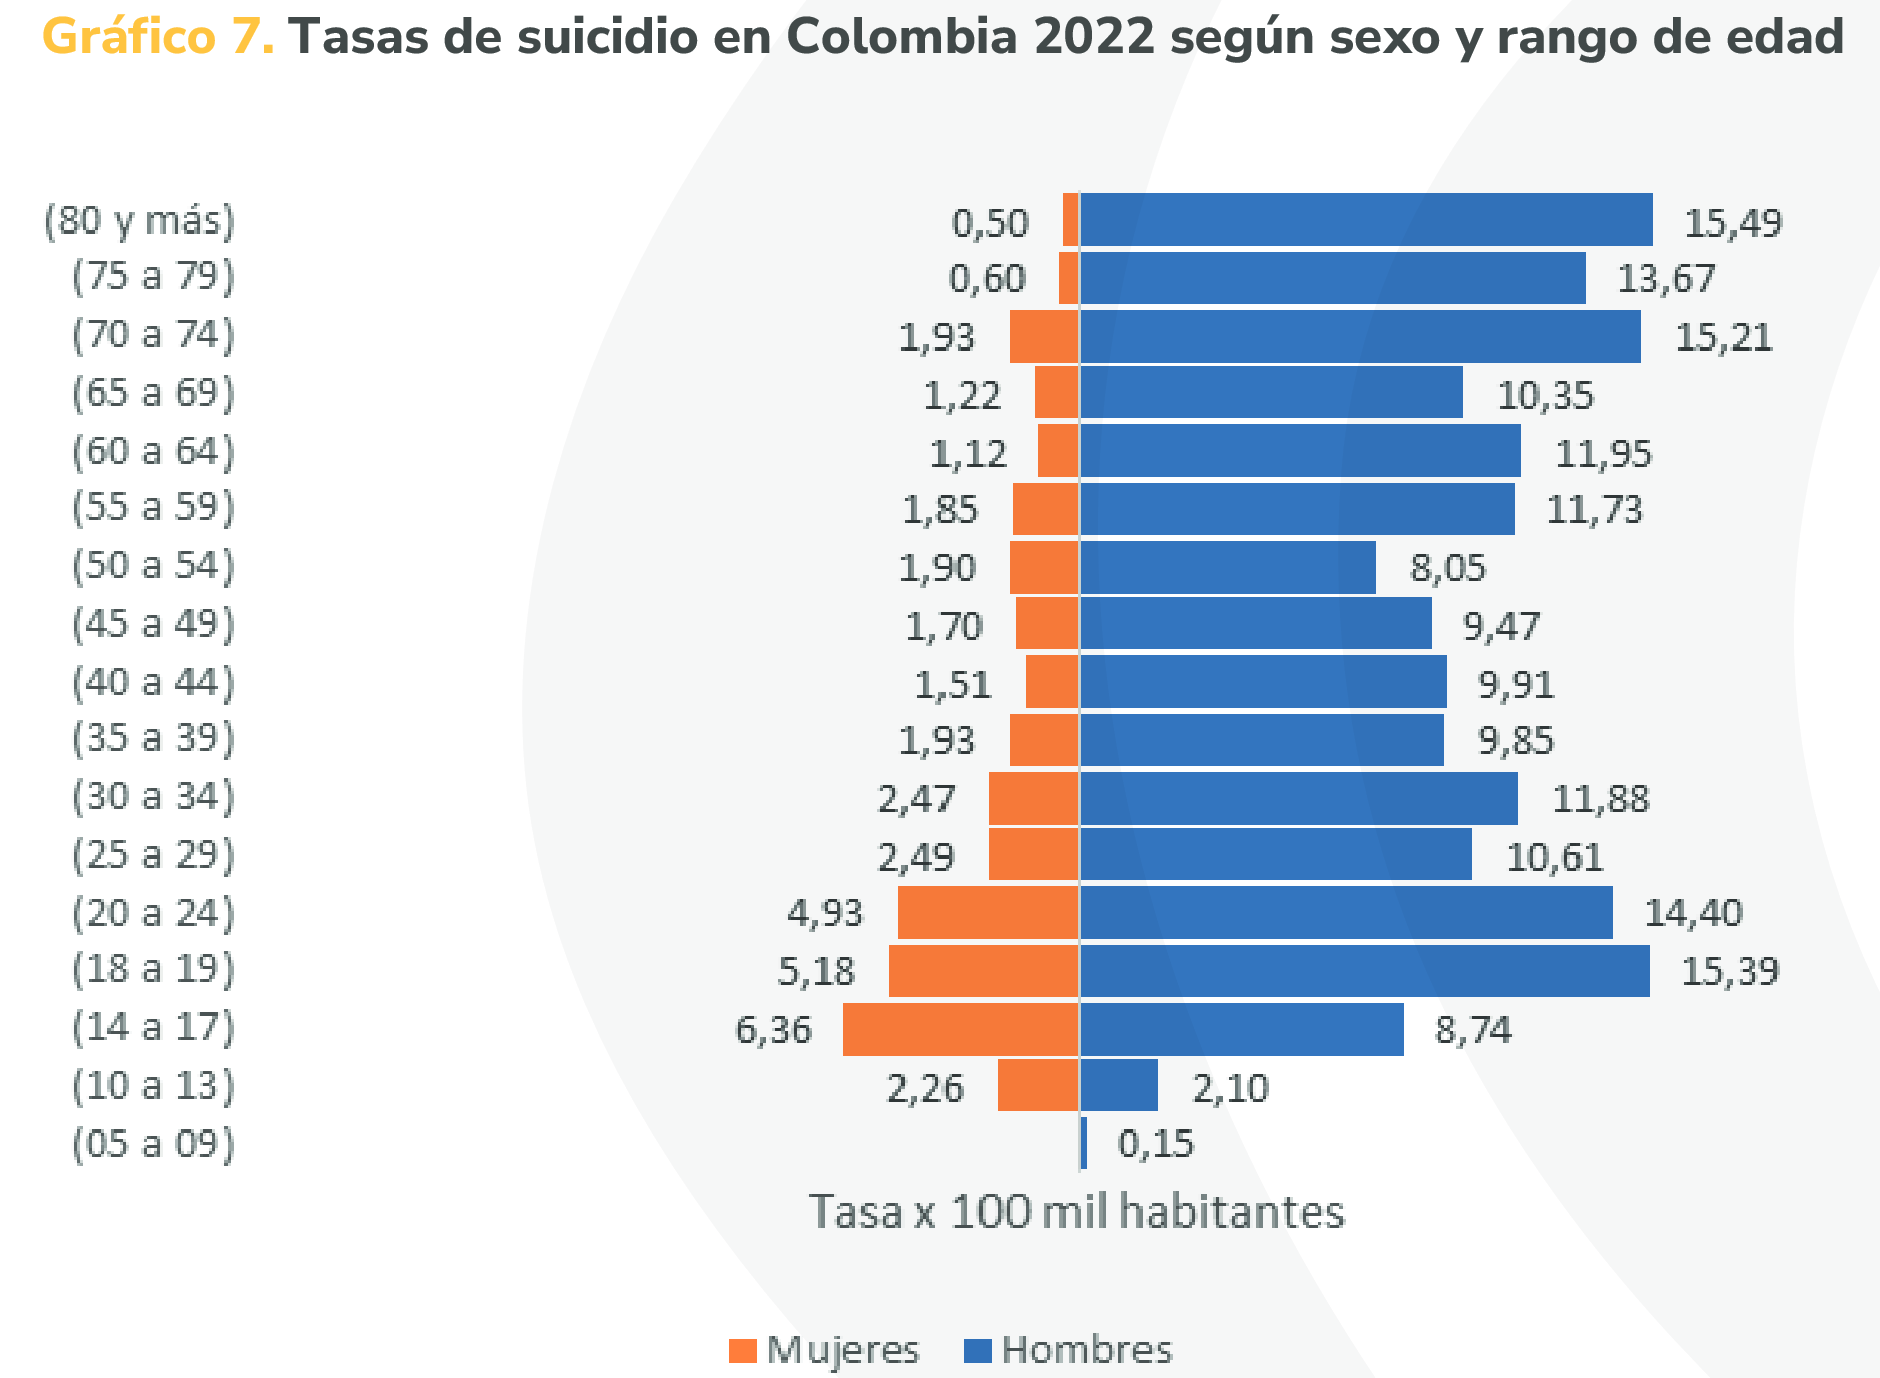
\includegraphics{suicidios.png}
\caption{Casos de suicidios Colombia}
\end{figure}

\begin{figure}
\centering
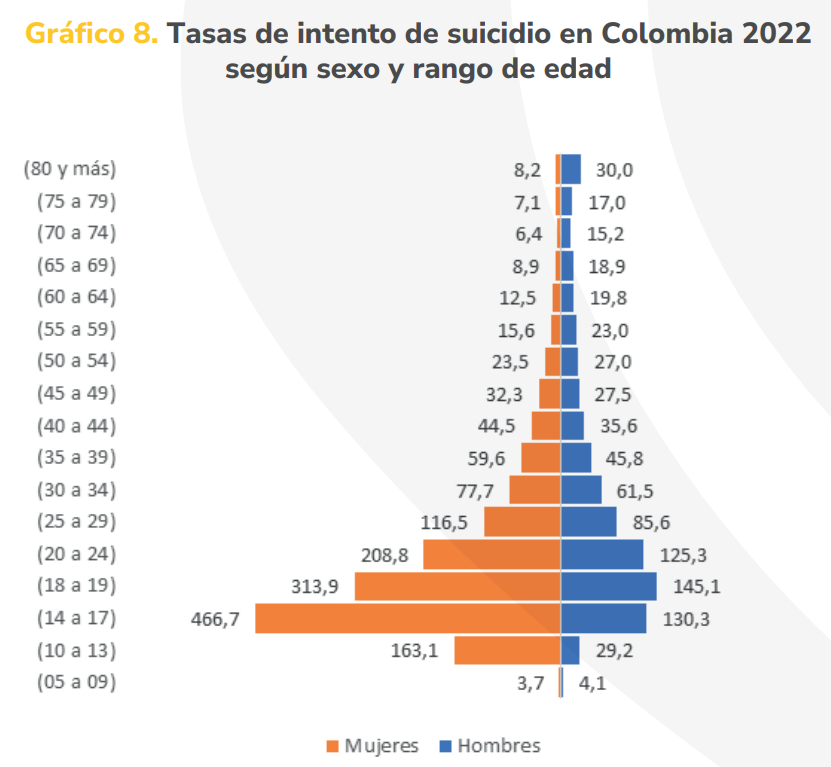
\includegraphics{intentos.png}
\caption{Casos de intentos de suicidio Colombia}
\end{figure}

La diferencia información proporcionada en el dataset de intentos de
suicidio y los casos de suicidio, podría deberse a que las mujeres
tienden a recurrir a servicios de ayuda anti-suicidios más que los
hombres, lo que puede ser de ayuda para que mueran menos personas de
este sector; sin embargo, al los hombres recurrir menos a estas ayudas,
sus tasas de suicidio son abrumadoramente mayores.

Además, la tendencia de los datos de intentos de suicidio se reflejan en
los casos de suicidio en las mujeres, algo que no ocurre de igual manera
con los hombres, siendo estas tasas bajan a los 50 años, pero
seguidamente vuelven a subir casi a su máximo, siendo este rango (18 -
24 \& 70 - 80+).

A partir de la información de los municipios, se puede observar la
incidencia de casos reportados en el Área Metropolitana de Bucaramanga y
alrededores. Algo que puede deberse a tener una mayor cantidad de
habitantes, y en el caso de municipios circundantes, debido a su
cercanía a la capital, los casos en ellos suelen ser más comúnmente
reportados.

En cuanto a los barrios de Bucaramanga, pese a que hay varios casos en
los que el barrio no fue registrado, se puede indicar una incidencia en
barrios como: Campo Hermoso, Provenza, Centro, Real de Minas y San
Francisco. Estos datos nos pueden indicar que es necesario que las
políticas que vayan encaminadas a tratar de reducir estos casos, le den
cierta prioridad a estos barrios para tratar de disminuir sus grandes
tasas de intentos de suicidio.

\subsection{Mecanismos de intento
suicida}\label{mecanismos-de-intento-suicida-1}

A partir de las gráficas generadas se puede observar que el mecanismo de
suicidio que es más ampliamente utilizado es el de intoxicación, seguido
por el uso de armas corto punzantes, quien a su vez está seguido de
lanzamiento al vacío y ahorcamiento.

Dentro de los casos de intoxicación se encuentra que los medicamentos
son las sustancias más ampliamente utilizadas, seguido de los
plaguicidas.

Estos resultados pueden deberse a que la intoxicación puede ser vista
como una alternativa más efectiva, menos dolorosa y más discreta que
otros métodos. Así como es fácilmente accesible, especialmente en el
caso de medicamentos y plaguicidas, lo que ayuda a que sea un método muy
recurrido.

El uso de armas corto punzantes y el salto al vacío son también
alternativas muy usadas. Lo que puede deberse a la facilidad para
obtener armas corto punzantes o acceder a un piso lo suficientemente
alto de un edificio.

\subsection{Factores desencadenantes}\label{factores-desencadenantes-1}

Es posible observar que los factores desencadenantes con mayor
incidencia son: problemas con la pareja, problemas familiares, problemas
económicos, problemas escolares y maltrato. Esto se debe a que son
factores que ejercen una mayor influencia sobre las emociones de las
personas.

El caso de los problemas de pareja y familiares se ven potenciados por
el hecho de que tanto la pareja como la familia suelen ser un entorno de
fuerte apoyo emocional. Esta dependencia emocional genera que las
personas puedan experimentar crisis severas ante conflictos con la
pareja o la familia.

Los problemas económicos generan una presión enorme en las personas, ya
que afectan la capacidad de cubrir necesidades básicas.

La presión académica suele ser un factor que puede generar estrés en
niños, adolescentes y jóvenes, en especial si viene acompañado de
grandes expectativas y miedo al fracaso.

El maltrato puede generar diversos traumas que pueden generar en las
personas que lo padecieron trastornos de ansiedad, baja autoestima y
depresión.

\subsection{Factores de riesgo}\label{factores-de-riesgo-1}

Es posible observar que los factores de riesgo con mayor incidencia en
los casos de intentos de suicidio son: trastornos psiquiátricos,
trastorno depresivo, ideación suicida persistente y consumo de
sustancias psicoactivas.

Los trastornos psiquiátricos y de depresión son productos de la
dificultad de las personas para manejar sus emociones, y deriva en un
aislamiento social que dificulta el que puedan acceder a ayuda.

La ideación suicida persistente es un factor que suele ser desapercibido
en etapas tempranas, pero puede volverse abrumador si no se interviene a
tiempo y llevar a disminuir la percepción del riesgo que implica el acto
suicida.

El consumo de sustancias psicoactivas suele deberse o relacionarse con
otros factores de riesgo y factores desencadenantes. Además de que estas
sustancias alteran enormemente la percepción y la capacidad de juicio de
quienes las consumen, quienes al ser incapaces de evaluar las
consecuencias de sus acciones, pueden ser más impulsivos ante
pensamientos suicidas.

\section{\texorpdfstring{\textbf{Conclusiones}}{Conclusiones}}\label{conclusiones}

El análisis de las tendencias mostradas por las gráficas permiten
comprender cuáles son los factores de mayor incidencia, los cuales
tienen prioridad de ser abordados. Las estrategias efectivas para
reducir esta problemática deben considerar una intervención integral
para abordar los factores demográficos, desencadenantes y de riesgo, así
como también los métodos de autolesión utilizados. A continuación se
presentan los factores a tener en cuenta para abordar la problemática:

\begin{itemize}
\item
  \textbf{Promoción de la salud mental:} Es necesario realizar campañas
  que puedan ayudar a concientizar sobre los problemas de salud mental,
  lo que ayudará a las personas a buscar la ayuda necesaria sin temor a
  ser juzgadas.

  Se pueden implementar programas que estén enfocados en adolescentes y
  jóvenes que puedan ayudarles a regular sus emociones y autoestima y
  manejar de mejor manera factores como la presión social y el estrés.
\item
  \textbf{Fortalecimiento de redes de apoyo:} La realización de
  programas que fomenten la orientación y comunicación en las relaciones
  familiares y de pareja es eficaz para prevenir conflictos que pueden
  resultar en impactos emocionales muy grandes que pueden terminar en
  tragedias como un intento de suicidio.

  También serían de utilidad programas que traten de ayudar a aliviar
  las presiones económicas en personas en las poblaciones más
  vulnerables, abordando cuestiones como la deuda y el desempleo. Lo que
  ayudaría a reducir el estrés y por ende el impacto emocional que el
  factor económico puede generar.
\item
  \textbf{Detección temprana y tratamiento oportuno:} Los resultados dan
  a entender la importancia de una detección temprana de factores
  desencadenantes y de riesgo, como trastornos psiquiátricos y
  depresivos, estrés por presión académica, maltrato en entornos
  familiares, escolares o de pareja, entre otros.

  Es importante capacitar a profesores en las escuelas y a trabajadores
  del sistema de salud para que sean capaces de detectar estos factores
  de riesgo, para que las personas, y en especial los adolescentes,
  puedan recibir una atención temprana para prevenir posibles casos
  futuros.
\item
  \textbf{Regulación y control de medios:} Dado al elevado uso de
  métodos como la intoxicación y el salto al vacío. Sería de gran ayuda
  regular la venta de medicamentos y plaguicidas para prevenir su uso
  como medio de autolesión. Así como también el promover medidas de
  seguridad en edificios altos, restringiendo el acceso a zonas
  peligrosas.
\item
  \textbf{Abordaje del consumo de sustancias psicoactivas:} Es necesario
  desarrollar iniciativas, especialmente enfocadas en adolescentes y
  jóvenes, que ayuden a desalentar el uso de sustancias psicoactivas,
  enfatizando en sus consecuencias para la salud mental.

  También es necesario ofrecer programas que ayuden a tratar el consumo
  de estas sustancias.
\end{itemize}

\section{\texorpdfstring{\textbf{Referencias}}{Referencias}}\label{referencias}

\begin{itemize}
\tightlist
\item
  \begin{enumerate}
  \def\labelenumi{\arabic{enumi}.}
  \setcounter{enumi}{85}
  \tightlist
  \item
    Intencion suicida sivigila enero 2016 a abril 2023 - semana
    epidemiológica 15 \textbar{} Datos Abiertos Colombia. (2023, May
    11).
    \url{https://www.datos.gov.co/Salud-y-Protecci-n-Social/86-Intencion-suicida-sivigila-enero-2016-a-abril-2/78wv-f29q/about_data}
  \end{enumerate}
\item
  EL SUICIDIO EN COLOMBIA: factores diferenciales entre mujeres y
  hombres. (s.~f.). En Observatoriomujeres.
  \url{https://observatoriomujeres.gov.co/archivos/Publicaciones/Publicacion_311.pdf}
\end{itemize}

\end{document}
